\documentclass[a4paper,11pt]{article}
\usepackage[left=2.5cm, right=2.5cm, top=1.5cm, bottom=1.5cm]{geometry}
\usepackage{graphicx}
\usepackage{amssymb}
\usepackage{amsmath}
\usepackage[procnames]{listings}
\usepackage{xcolor}
\usepackage[active,tightpage]{preview}
\usepackage{hyperref}

\hypersetup{ %color attributes of citation, link, etc.
    colorlinks=true,
    linkcolor=blue,
    filecolor=gray,
    urlcolor=blue,
    citecolor=blue,
}

\setlength{\parindent}{0pt}

\renewcommand{\PreviewBorder}{1in}
\newcommand{\Newpage}{\end{preview}\begin{preview}}
\newcommand{\matlab}{\textsc{Matlab}} %very important and totally necessary addition
\newcommand{\parallelsum}{\mathbin{\!/\mkern-5mu/\!}}

\newcommand\Item[1][]{%
  \ifx\relax#1\relax  \item \else \item[#1] \fi
  \abovedisplayskip=0pt\abovedisplayshortskip=0pt~\vspace*{-\baselineskip}}

%'codify' text for snippets
\usepackage{xcolor}
\definecolor{codegray}{gray}{1}
\newcommand{\code}[1]{\colorbox{codegray}{\texttt{#1}}}

\definecolor{keywords}{RGB}{255,0,90}
\definecolor{comments}{RGB}{0,0,113}
\definecolor{p_red}{RGB}{160,0,0}
\definecolor{p_green}{RGB}{0,150,0} 
\lstset{language=Python, 
        basicstyle=\ttfamily\small, 
        keywordstyle=\color{keywords},
        commentstyle=\color{comments},
        stringstyle=\color{p_red},
        showstringspaces=false,
        identifierstyle=\color{p_green},
		procnamekeys={def,class}}

\graphicspath{ {./images/} }
           
\begin{document}
\begin{preview}
\title{\LARGE{\textbf{ENGR222 Assignment 2}}}
\author{Niels Clayton : 300437590}
\date{}
\maketitle
\hrule

\begin{enumerate}
    \item The following questions are concerned with the function
    $$ f(x,y) = -2x^3 + 3x^2y + 2y^3 - 9y +5$$

    \begin{enumerate}
        \item Determine the first order partial derivative of $f(x, y)$
        \begin{align*}
            f_x &= -6x^2 + 6xy \\
            f_y &=  6y^2 + 3x^2 - 9
        \end{align*}
    
        \item Determine the second order partial derivatives of $f(x, y)$
        \begin{align*}
            f_{xx} &= -12x + 6y\\
            f_{yy} &= 12y \\
            f_{xy} &= 6x\\
        \end{align*}
    
        \item Find all of the critical points of $f(x, y)\\$

            $\mathrm{By \; inspection \; we \; know \;}  (x=y= -1,1)\\\\$
            Let $x = 0\\$

            \begin{align*}
                f_{x} &= 0 \\
                f_{y} &= 6y^2 - 9 = 0\\
                \therefore y &= \sqrt{\frac{9}{6}} = \sqrt{\frac{3}{2}}\\\\
            \end{align*}

            Let $y = 0\\$

            \begin{align*}
                f_{x} &= -6x^2 = 0 \\
                f_{y} &= 3x^2 -9 
            \end{align*}
            \begin{center}
                No solution for $x$ when $y=0$ \newline
            \end{center}

            The critical points are $\rightarrow [(1,1), \; (-1,-1), \; (0, \sqrt{\frac{3}{2}})]$

        \item Classify the critical point $(0,\sqrt{\frac{3}{2}})$
        
        \begin{align*}
            D &= f_{xx}(0, \sqrt{\frac{3}{2}}) \times f_{yy}(0, \sqrt{\frac{3}{2}}) - f_{xy}^2 (0, \sqrt{\frac{3}{2}})\\\\
            f_{xx}(0, \sqrt{\frac{3}{2}}) &= 3\sqrt{6}\\
            f_{yy}(0, \sqrt{\frac{3}{2}}) &= 6\sqrt{6}\\
            f_{xy}(0, \sqrt{\frac{3}{2}}) &= 0\\\\
            D &= 3\sqrt{6} \times 6\sqrt{6} - 0^2 = 108
        \end{align*}
        Since $D  > 0$ and $f_{xx} > 0$ we know this critical point is a local minimum\\
    
    \end{enumerate}

    \item Quick questions
    
    \begin{enumerate}
        \item Determine the directional derivative of $f(x,y,z) = e^x \cdot \cos(y) \cdot (1-z)^2$ in direction $\bar{u} =  (0.36, 0.48, 0.8)$ from the origin:
        
        \begin{align*}
            D_u f(x_0,y_0,z_0) &= f_x(x_0,y_0,z_0)\bar{u}_1 + f_y(x_0,y_0,z_0)\bar{u}_2 + f_z(x_0,y_0,z_0)\bar{u}_3\\\\
            f_{x} &= e^{x}cos(y)(1-z)^{2} \\
            f_{y} &= -e^{x}sin(y)(1-z)^2 \\
            f_{z} &= e^{x}cos(y)(2z - 2)\\\\
            f_x(0,0,0) &= 1\cdot 1 \cdot1 = 1\\
            f_y(0,0,0) &= -1 \cdot 0 \cdot 1 = 0\\
            f_z(0,0,0) &= 1 \cdot 1 \cdot -2 = -2\\\\
            D_u f(0,0,0) &= 0.36 -1.6 = -1.24\\
        \end{align*}

        \item Determine the local linear approximation of $f(x, y, z) = (1+x)(1-y^2)(1-z)^2$ at the point $(1, 2, 3)$
        
        \begin{align*}
            L(x,y,z) &= f(x_0, y_0, z_0) + f_x(x_0, y_0, z_0)(x-x_0) + f_y(x_0, y_0, z_0)(y-y_0) + f_z(x_0, y_0, z_0)(z-z_0)\\\\
            f_{x}        & = (1-y^2)(1-z)^2                               \\
            f_{y}        & = (1+x)(-2y)(1-z)^2                            \\
            f_{z}        & = 2(1+x)(1-y^2)(z-1)                           \\\\
            f(1,2,3)     & = (1+1)(1-2^2)(1-3)^2=-24                      \\  
            f_{x}(1,2,3) & = (1-2^2)(1-3)^2=-12                           \\
            f_{y}(1,2,3) & = (1+1)(-2(2))(1-3)^2=-32                      \\
            f_{z}(1,2,3) & = 2(1+1)(1-2^2)(3-1)=-24                       \\\\
            L(1,2,3)     & = -24 -12(x - 1) -32(y - 2) -24(z - 3)\\
            L (1,2,3)    & = 124-12x-32y-24z\\
        \end{align*}
    
        \item Determine the 2nd degree Taylor polynomial of $ f(x,y) = e^{-x^2}e^{-y^2} $ as the point (1,1)

        \begin{align*}
            L(x,y) &= f(x_0, y_0) + f_x(x_0, y_0)(x-x_0) + f_y(x_0, y_0)(y-y_0)\\
            p_2(x,y) &= L(x,y) + \frac{1}{2}\left[ f_{xx}(x_0, y_0)(x-x_0)^2 + 2f_{xy}(x_0, y_0)(x-x_0)(y-y_0) + f_{yy}(x_0, y_0)(y-y_0)^2 \right]\\\\
            f_x     &= (-2x) e^{-x^2}e^{-y^2}             \\
            f_y     &= (-2y) e^{-x^2}e^{-y^2}             \\\\
            f_{xx}  &= (4 x^2 - 2) e^{-x^2 - y^2}         \\
            f_{yy}  &= (4 y^2 - 2) e^{-x^2 - y^2}         \\
            f_{xy}  &= (4xy) e^{-x^2}e^{-y^2}             \\\\
            L(1,1)  &= e^{-2} -2e^{-2}(x-1) - 2e^{-2}(y-1) = e^{-2}(5-2x-2y)\\
            p_2(1,1)&= e^{-2}(5-2x-2y) + \frac{1}{2} \left[  2e^{-2}(x-2)^2 + 2e^{-2}(y-2)^2 + 8e^{-2}(x-1)(y-1)\right] \\
                    &= e^{-2}(x^2 + y^2 -8x -8y +4xy +11)
        \end{align*}

        \item Determine the gradient of $f(x,y) = x^3+y^3-4x-2y$ along the curve \\$(x(t), y(t)) = (t^3 - 2t, t^2)$ when $t=1$
        
        \begin{align*}
            \bigtriangledown f(x,y) &= f_x(x,y)\textbf{i} + f_y(x,y)\textbf{j}\\\\
            f_x &= 3x^2 -4\\
            f_y &= 3y^2 -2\\
            \therefore \bigtriangledown f(x,y) &= (3x^2 -4)\textbf{i} + (3y^2 -2)\textbf{j}\\\\
            (x(1),y(1)) &= (-1,1)\\
            \bigtriangledown f(-1,1) &= f_x(-1,1)\textbf{i} + f_y(-1,1)\textbf{j}\\
            &= -1 \textbf{i} + 1 \textbf{j}
        \end{align*}

        \item Determine the tangent plane to the surface $z = x^2 + xy -y^4$ at the point $(x,y)=(2,1)$
        \begin{align*}
            F(x,y,z) &= z - x^2 - xy + y^4 = 0\\\\
            \mathrm{Find \; } &z \mathrm{\; at\; the \; point \;} (x,y) = (2,1)\\
            z &= 2^2 + 2 -1^4=5\\\\
            \bigtriangledown F(x,y,z) &= (-2x-y) \textbf{i} + (4y^3-x)\textbf{j} + \textbf{k}\\
            \bigtriangledown F(2,1,5) &= -5\textbf{i} + 2\textbf{j} + \textbf{k}\\\\
            \mathrm{Tangent Plane} &= -5(x-2) + 2(y-1) + (z-5)\\
            z &= 5x -2y -3
        \end{align*}
    
    \end{enumerate}

    \item Double Integrals
    
    \begin{enumerate}

        \item Determine the integral of $f(x,y) = e^{-x}\cos(y)$ over the rectangular region \\$R = {(x,y) : x \in [0,2], y \in [\frac{-\pi}{2}, \frac{\pi}{2}]}$'
        
        \begin{align*}
            &\int_{-\pi/2}^{\pi/2} \int_{0}^{2} e^{-x}\cos(y) \,dx \,dy\\\\
            &= \int_{-\pi/2}^{\pi/2} \cos(y) \int_{0}^{2} e^{-x} \,dx \,dy\\
            &= \int_{-\pi/2}^{\pi/2} \cos(y) \Big| -e^{-x} \Big|_{x = 0}^{x = 2} \,dy\\
            &= \int_{-\pi/2}^{\pi/2} \cos(y) (-e^{-2} - -e^0) \,dy\\\\
            &= \int_{-\pi/2}^{\pi/2} \cos(y) (-e^{-2} +1) \,dy\\
            &= (-e^{-2} +1) \Big| \sin(y) \Big|_{y = -\pi/2}^{y = \pi/2}\\
            &= (-e^{-2} +1) (\sin(\pi/2) - \sin(-\pi/2))\\\\
            &= -2e^{-2} +2\\
        \end{align*}
    
        \item Determine the integral of $f(x,y)=\sin(x+y)$ over the triangular region for which $ x \geq 0, \; y \geq 0 $ and $ x+y \leq \pi $
        
        \begin{align*}
            &\int_{0}^{\pi} \int_{0}^{\pi - x} \sin(x+y) \,dy  \,dx \\\\
            &= \int_{0}^{\pi} \Big|-\cos(x+y) \Big|_{0}^{\pi - x}  \,dx \\
            &= \int_{0}^{\pi} -\cos(\pi) + cos(x) \,dx \\
            &= \int_{0}^{\pi} 1 + \cos(x) \,dx \\\\
            &= \Big| x +\sin(x) \Big|_{0}^{\pi} \\
            &= (\pi + \sin(\pi)) - (0 +\sin(0)) \\
            &= \pi
        \end{align*}

        \item Determine the area of the region $R = \{(x,y) : e^{y/3} \leq x \leq 10+\sin(y), y \in [0,5]\}$ 
        
        \begin{align*}
            &\int_{0}^{5} \int_{e^{y/3}}^{10+\sin(y)} \,dx  \,dy \\\\
            &\int_{0}^{5} \Big| x  \Big|_{e^{y/3}}^{10+\sin(y)} \,dy \\
            &\int_{0}^{5}  10+\sin(y) - e^{y/3} \,dy \\\\
            &= \Big| 10y -\cos(y) - 3e^{y/3} \Big|_{0}^{5} \\
            &= 50 -\cos(5) - 3e^{5/3} + \cos(0) + 3e^{0} \\
            &= 37.832 \\
        \end{align*}

        \item Determine the average of $f(x,y) = 3y-2x$ over the region \\$R = \{ (x,y) : 0 \leq y \leq 4-x^2, x \in [-2,2] \}$
        
        \begin{align*}
            \mu &= \frac{1}{|R|} \iint_R f(x,y) dA\\\\
            |R| &= \int_{-2}^{2} \int_{0}^{4-x^2} \,dy  \,dx \\
                &= \int_{-2}^{2} \big| y \Big|_{0}^{4-x^2} \,dx \\
                &= \int_{-2}^{2} 4-x^2 \,dx \\\\
                &= \Big| 4x - \frac{x^3}{3} \Big|_{-2}^{2} \\
                &= 8 - \frac{2^3}{3} + 8 - \frac{2^3}{3} \\ 
                &= \frac{32}{3}\\\\
                &\int_{-2}^{2} \int_{0}^{4-x^2} 3y - 2x \,dy  \,dx \\
                &= \int_{-2}^{2} \Big| \frac{3y^2}{2} - 2xy \Big|_{0}^{4-x^2} \,dx \\
                &= \int_{-2}^{2} \frac{3(4-x^2)^2}{2} - 2x(4-x^2) \,dx \\
                &= \int_{-2}^{2} \frac{3x^4}{2} + 2x^3 - 12x^2 - 8x + 24 \,dx \\\\
                &= \int_{-2}^{2} \frac{3x^5}{10} + \frac{x^4}{2} - 4x^3 - 4x^2 + 24x  \\
                &= \Big| \frac{3x^5}{10} + \frac{x^4}{2} - 4x^3 - 4x^2 + 24x \Big|_{-2}^{2} \\
                &= (\frac{3(2)^5}{10} + \frac{(2)^4}{2} - 4(2)^3 - 4(2)^2 + 24(2)) - (\frac{3(-2)^5}{10} + \frac{(-2)^4}{2} - 4(-2)^3 - 4(-2)^2 + 24(-2))\\
                &= \frac{256}{5}\\\\
            \mu &= \frac{\frac{256}{5}}{\frac{32}{3}} \\
                &= \frac{24}{5} = 4.8
        \end{align*}

        \item Determine the surface area of the surface described by $z = \sqrt{9 - x^2}$ over the region $R = \{ (x,y) : 0 \leq y \leq x, x \in [0,3] \}$ 
        
        \begin{align*}
            \mathrm{Surface \; Area \;} &= \iint_R \sqrt{ f_x(x,y)^2 + f_y(x,y)^2 +1} dA\\\\
            \mathrm{Integrand} &= \sqrt{ f_x(x,y)^2 + f_y(x,y)^2 +1}\\\\
            f_x &= -\frac{x}{\sqrt{9 - x^2}}\\
            f_y &= 0 \\\\
            \mathrm{Integrand} &= \sqrt{ \left(-\frac{x}{\sqrt{9 - x^2}}\right)^2 +1}\\\\
            &= \sqrt{ \frac{x^2}{9-x^2} +1} = \frac{3}{\sqrt{9-x^2}}\\\\
            \mathrm{Surface \; Area \;} &= \int_{0}^{3} \int_{0}^{x} \frac{3}{\sqrt{9-x^2}} \,dy  \,dx \\ 
            &= \int_{0}^{3} \Big| \left( \frac{3}{\sqrt{9-x^2}} \right) y \Big|_{0}^{x}  \,dx \\
            &= \int_{0}^{3} \left( \frac{3}{\sqrt{9-x^2}} \right) x  \,dx \\\\
            &= \Big| -3\sqrt{9-x^2} \Big|_{0}^{3}\\
            &= -3\sqrt{0} + 3\sqrt{9}\\
            &= 9\\
        \end{align*}
    \end{enumerate}

    \item Lab Questions
    
    \begin{enumerate}
        \item investigate the numerical approximation of a derivative
        \begin{enumerate}
            \item Estimate the numerical derivative of $f(x) = e^{\cos(\pi x^2)}$ at the point $x = 1/\sqrt{2}$ \\
            Estimate the derivative via: $$ \frac{df}{dx} \approx \frac{f(x +h) - f(x)}{h}$$
            
            for a range of step sizes $h$ plot the error verses the step size: 
            \begin{center}
                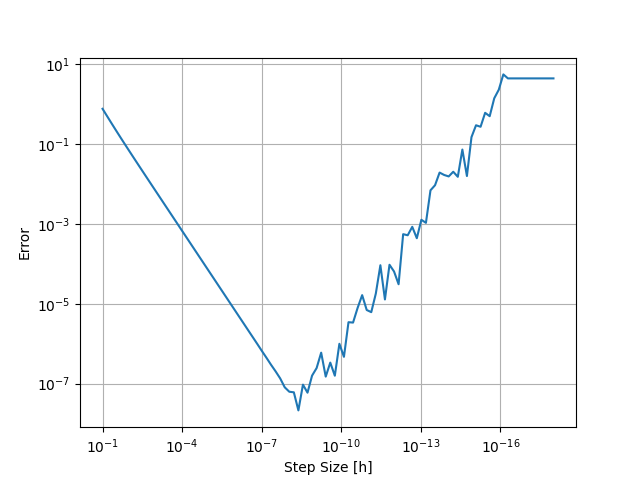
\includegraphics[width = 0.8\textwidth]{Figure_1.png}
            \end{center}

            The minimum error of \code{2.134e-08} was achieved with a step size of \code{4.132e-09}\\\\

            \item Estimate the numerical derivative of $f(x) = e^{\cos(\pi x^2)}$ at the point $x = 1/\sqrt{2}$ \\
            Estimate the derivative via: 
            
            $$ \frac{df}{dx} \approx \frac{f(x +h) - f(x-h)}{2h}$$
            
            for a range of step sizes $h$ plot the error verses the step size: 
            \begin{center}
                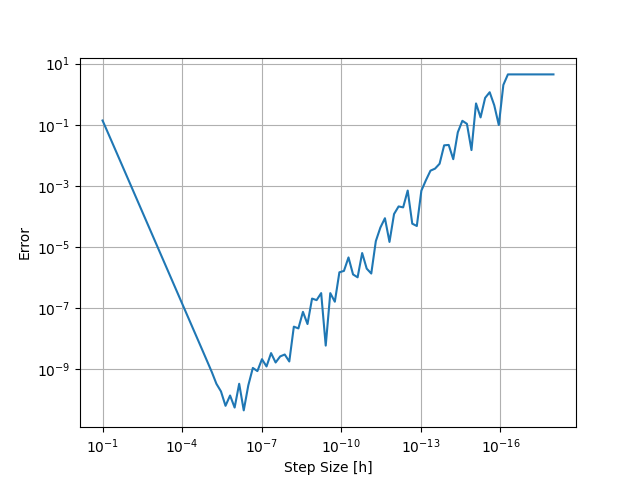
\includegraphics[width = 0.8\textwidth]{Figure_2.png}
            \end{center}

            The minimum error of \code{4.407e-11} was achieved with a step size of \code{4.75e-07}\\\\

            \item Estimate the numerical second derivative of $f(x) = e^{\cos(\pi x^2)}$ at the point $x = 1/\sqrt{2}$ \\
            Estimate the second derivative via: 
            
            $$ \frac{d^2f}{dx^2} \approx \frac{f(x +h) -2f(x) + f(x-h)}{h^2}$$
            
            for a range of step sizes $h$ plot the error verses the step size: 
            \begin{center}
                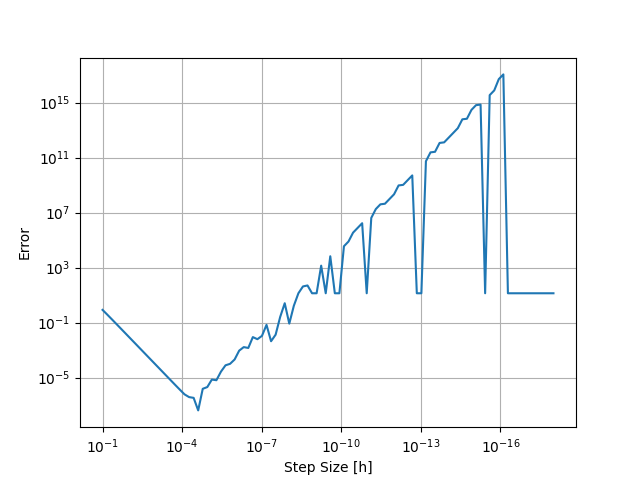
\includegraphics[width = 0.8\textwidth]{Figure_3.png}
            \end{center}

            The minimum error of \code{4.08e-08} was achieved with a step size of \code{2.477e-05}\\\\

        \end{enumerate}

        \item investigate the numerical approximation of an integral
        
        \begin{enumerate}
            \item Numerically integrate the following integral using the  trapezoidal rule, with sub-intervals of $n = 10,20,40,80,160$
            $$ \int_{0}^{10} xe^{-\sqrt{x}} \,dx $$
            
            The following is the numerical integral evaluations:\\\\
            \texttt{For a subinterval of 10 the integral is 4.608\\
            For a subinterval of 20 the integral is 4.652\\
            For a subinterval of 40 the integral is 4.664\\
            For a subinterval of 80 the integral is 4.668\\
            For a subinterval of 160 the integral is 4.669\\\\}

        \item Numerically integrate the following integral using the  Simpson rule, with sub-intervals of $n = 10,20,40,80,160$
        $$ \int_{0}^{10} xe^{-\sqrt{x}} \,dx $$

        The following is the numerical integral evaluations:\\\\
        \texttt{For a sub-interval of 10 the integral is 4.657102287466295\\
        For a sub-interval of 20 the integral is 4.666621390508981\\
        For a sub-interval of 40 the integral is 4.668462546387442\\
        For a sub-interval of 80 the integral is 4.668804644613161\\
        For a sub-interval of 160 the integral is 4.668866774081337\\\\}
        I am comfortable estimating that that 4 digits are correct. This this due to the speed of conversion of the Simpson's rule compared to the trapezoidal rule.\\\\

        \item Use the quad function from scipy.integrate to estimate the value of the integrals:

        $$ \int_{0}^{10} xe^{-\sqrt{x}}\,dx \; , \;\;\;\int_{0}^{100} xe^{-\sqrt{x}} \,dx \; , \;\;\; \int_{0}^{1000} xe^{-\sqrt{x}} \,dx \;\;\; $$
        
        The evaluation of these integrals is as follows:\\\\
        \texttt{At the upper bound of 10.0 the integral evaluates to 4.668880328350931\\
        At the upper bound of 100.0 the integral evaluates to 11.875967391881685\\
        At the upper bound of 1000.0 the integral evaluates to 11.999999998713989\\\\}

        This appears to converge to a value of 12.\\

        Now evaluate the following integral:\\
        $$ \int_{0}^{\infty} xe^{-\sqrt{x}}\,dx $$

        This evaluates to:\\
        \texttt{At an infinite upper bound the integral evaluates to 12.000000000094914}

        \end{enumerate}

    \end{enumerate}
    \section*{Lab Code}
    \lstinputlisting{lab/lab_questions.py}
\end{enumerate}
\end{preview}
\end{document}